A l'issue de la phase d'analyse, le code est disponible sous la forme d'une liste de \pyinline{StructureNode} (figure \ref{fig:parse_exemple}). C'est à partir de cette liste que sera produit le code assembleur et le code binaire associé.

L'ensemble des classes décrites ci-dessous font l'objet d'un transtypage permettant d'afficher celles-ci sous la forme d'une chaîne de caractères. 

\subsubsection{Classe StructureNode}

\begin{figure}[h!]
	\centering
	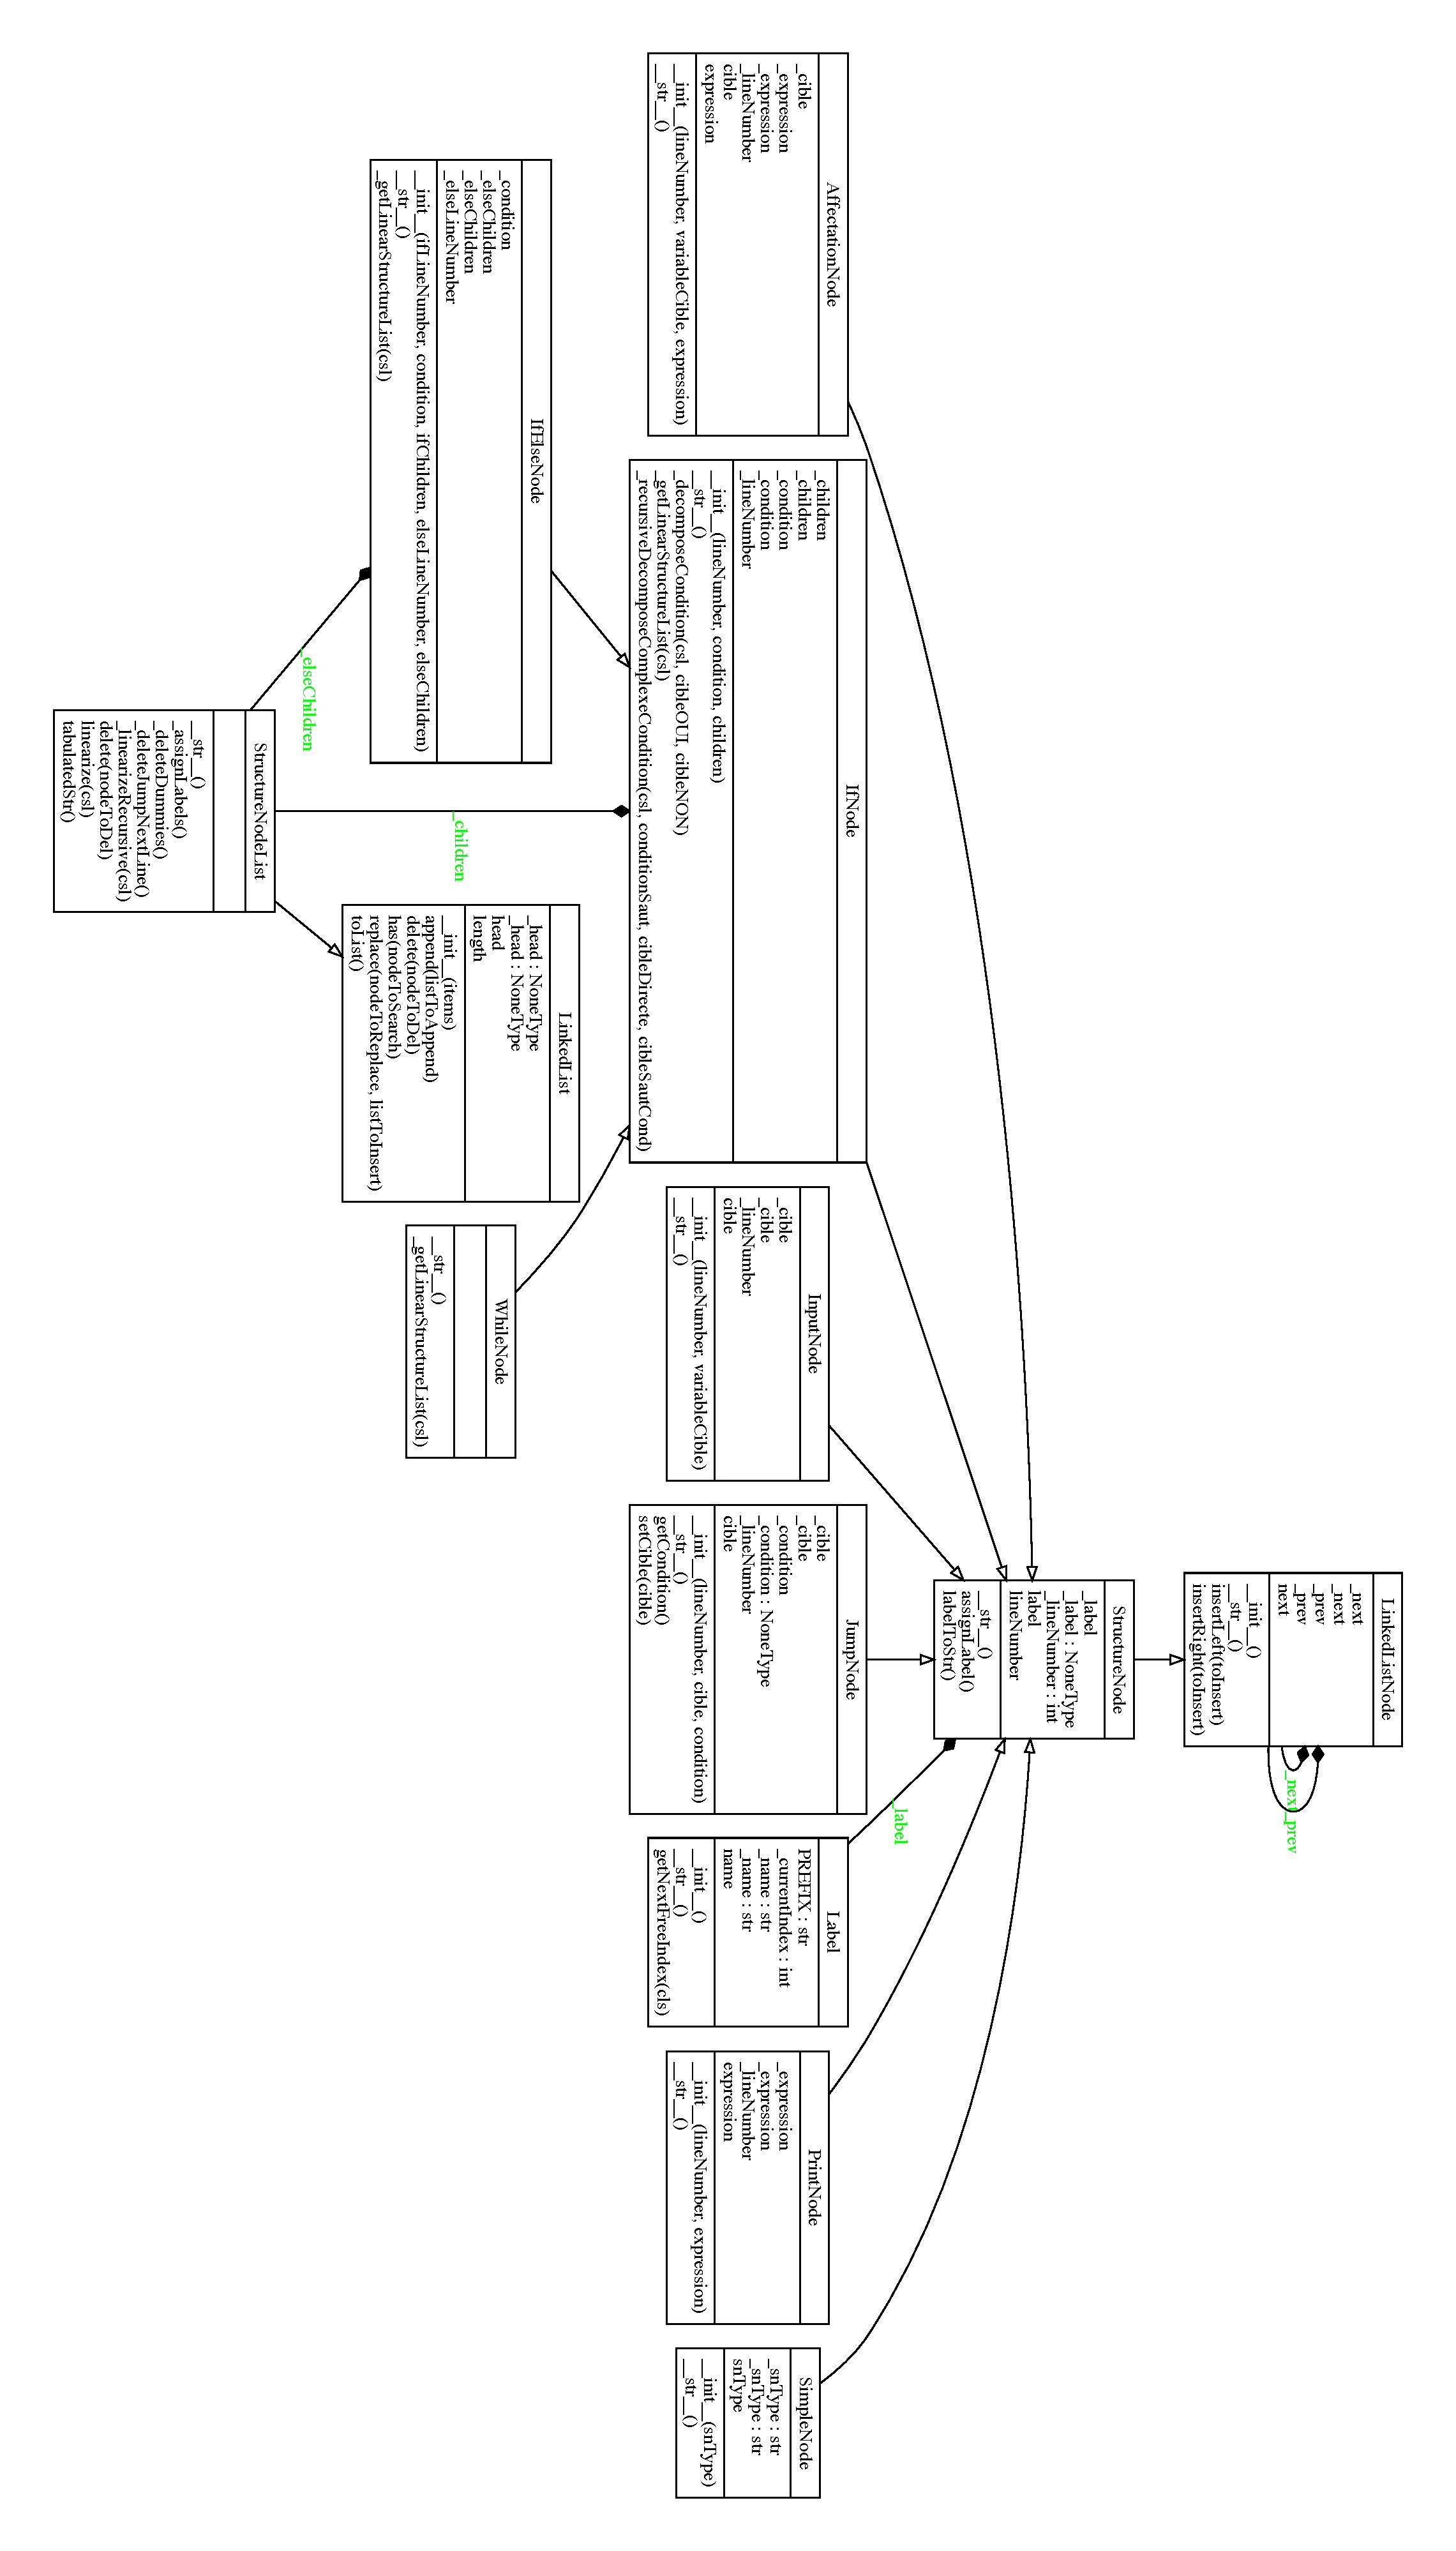
\includegraphics[height=25cm]{./Pictures/StructureNode.pdf}
	\caption{\label{fig:class_StructureNode}Diagramme de classes - StructureNode}
\end{figure}

Les classes héritées de \pyinline{StructureNode} sont présentées sur la figure \ref{fig:class_StructureNode}. On remarquera que les \pyinline{StructureNode} peuvent être des structures de données récursives, les n\oe uds de type \pyinline{IfNode}, \pyinline{IfElseNode} et \pyinline{WhileNode} ayant pour attribut \pyinline{_children} de type \pyinline{StructureNodeList}.

La classe \pyinline{StructureNode} est en particulier en charge d'assurer la linéarisation des boucles \pyinline{while} et des branchements \pyinline{if} en une série de sauts conditionnels ou inconditionnels
avec la méthode \pyinline{getLinearStructureList(csl)} où \pyinline{csl} est une liste de chaine de caractères correspondant aux symboles de comparaison disponibles dans le modèle de processeur retenu (\ref{sec:processeur}). Elle peut faire appelle le cas échéant aux méthodes des classes \pyinline{ComparisonExpressionNode} et \pyinline{LogicExpressionNode} afin d'adapter les expressions logiques en conséquence.

\clearpage

\subsubsection{Classes ArithmeticExpressionNode, LogicExpressionNode et ComparisonExpressionNode}

Les conditions des branchements \pyinline{if else} ou les arrêts de boucle \pyinline{while} sont implémentées comme des attributs (\pyinline{_condition}) de n\oe uds de type \pyinline{IfNode}, \pyinline{IfElseNode} et \pyinline{WhileNode}. Elles sont associées à des instances des classes \pyinline{LogicExpressionNode} ou \pyinline{ComparisonExpressionNode}.

\begin{figure}[h!]
	\centering
	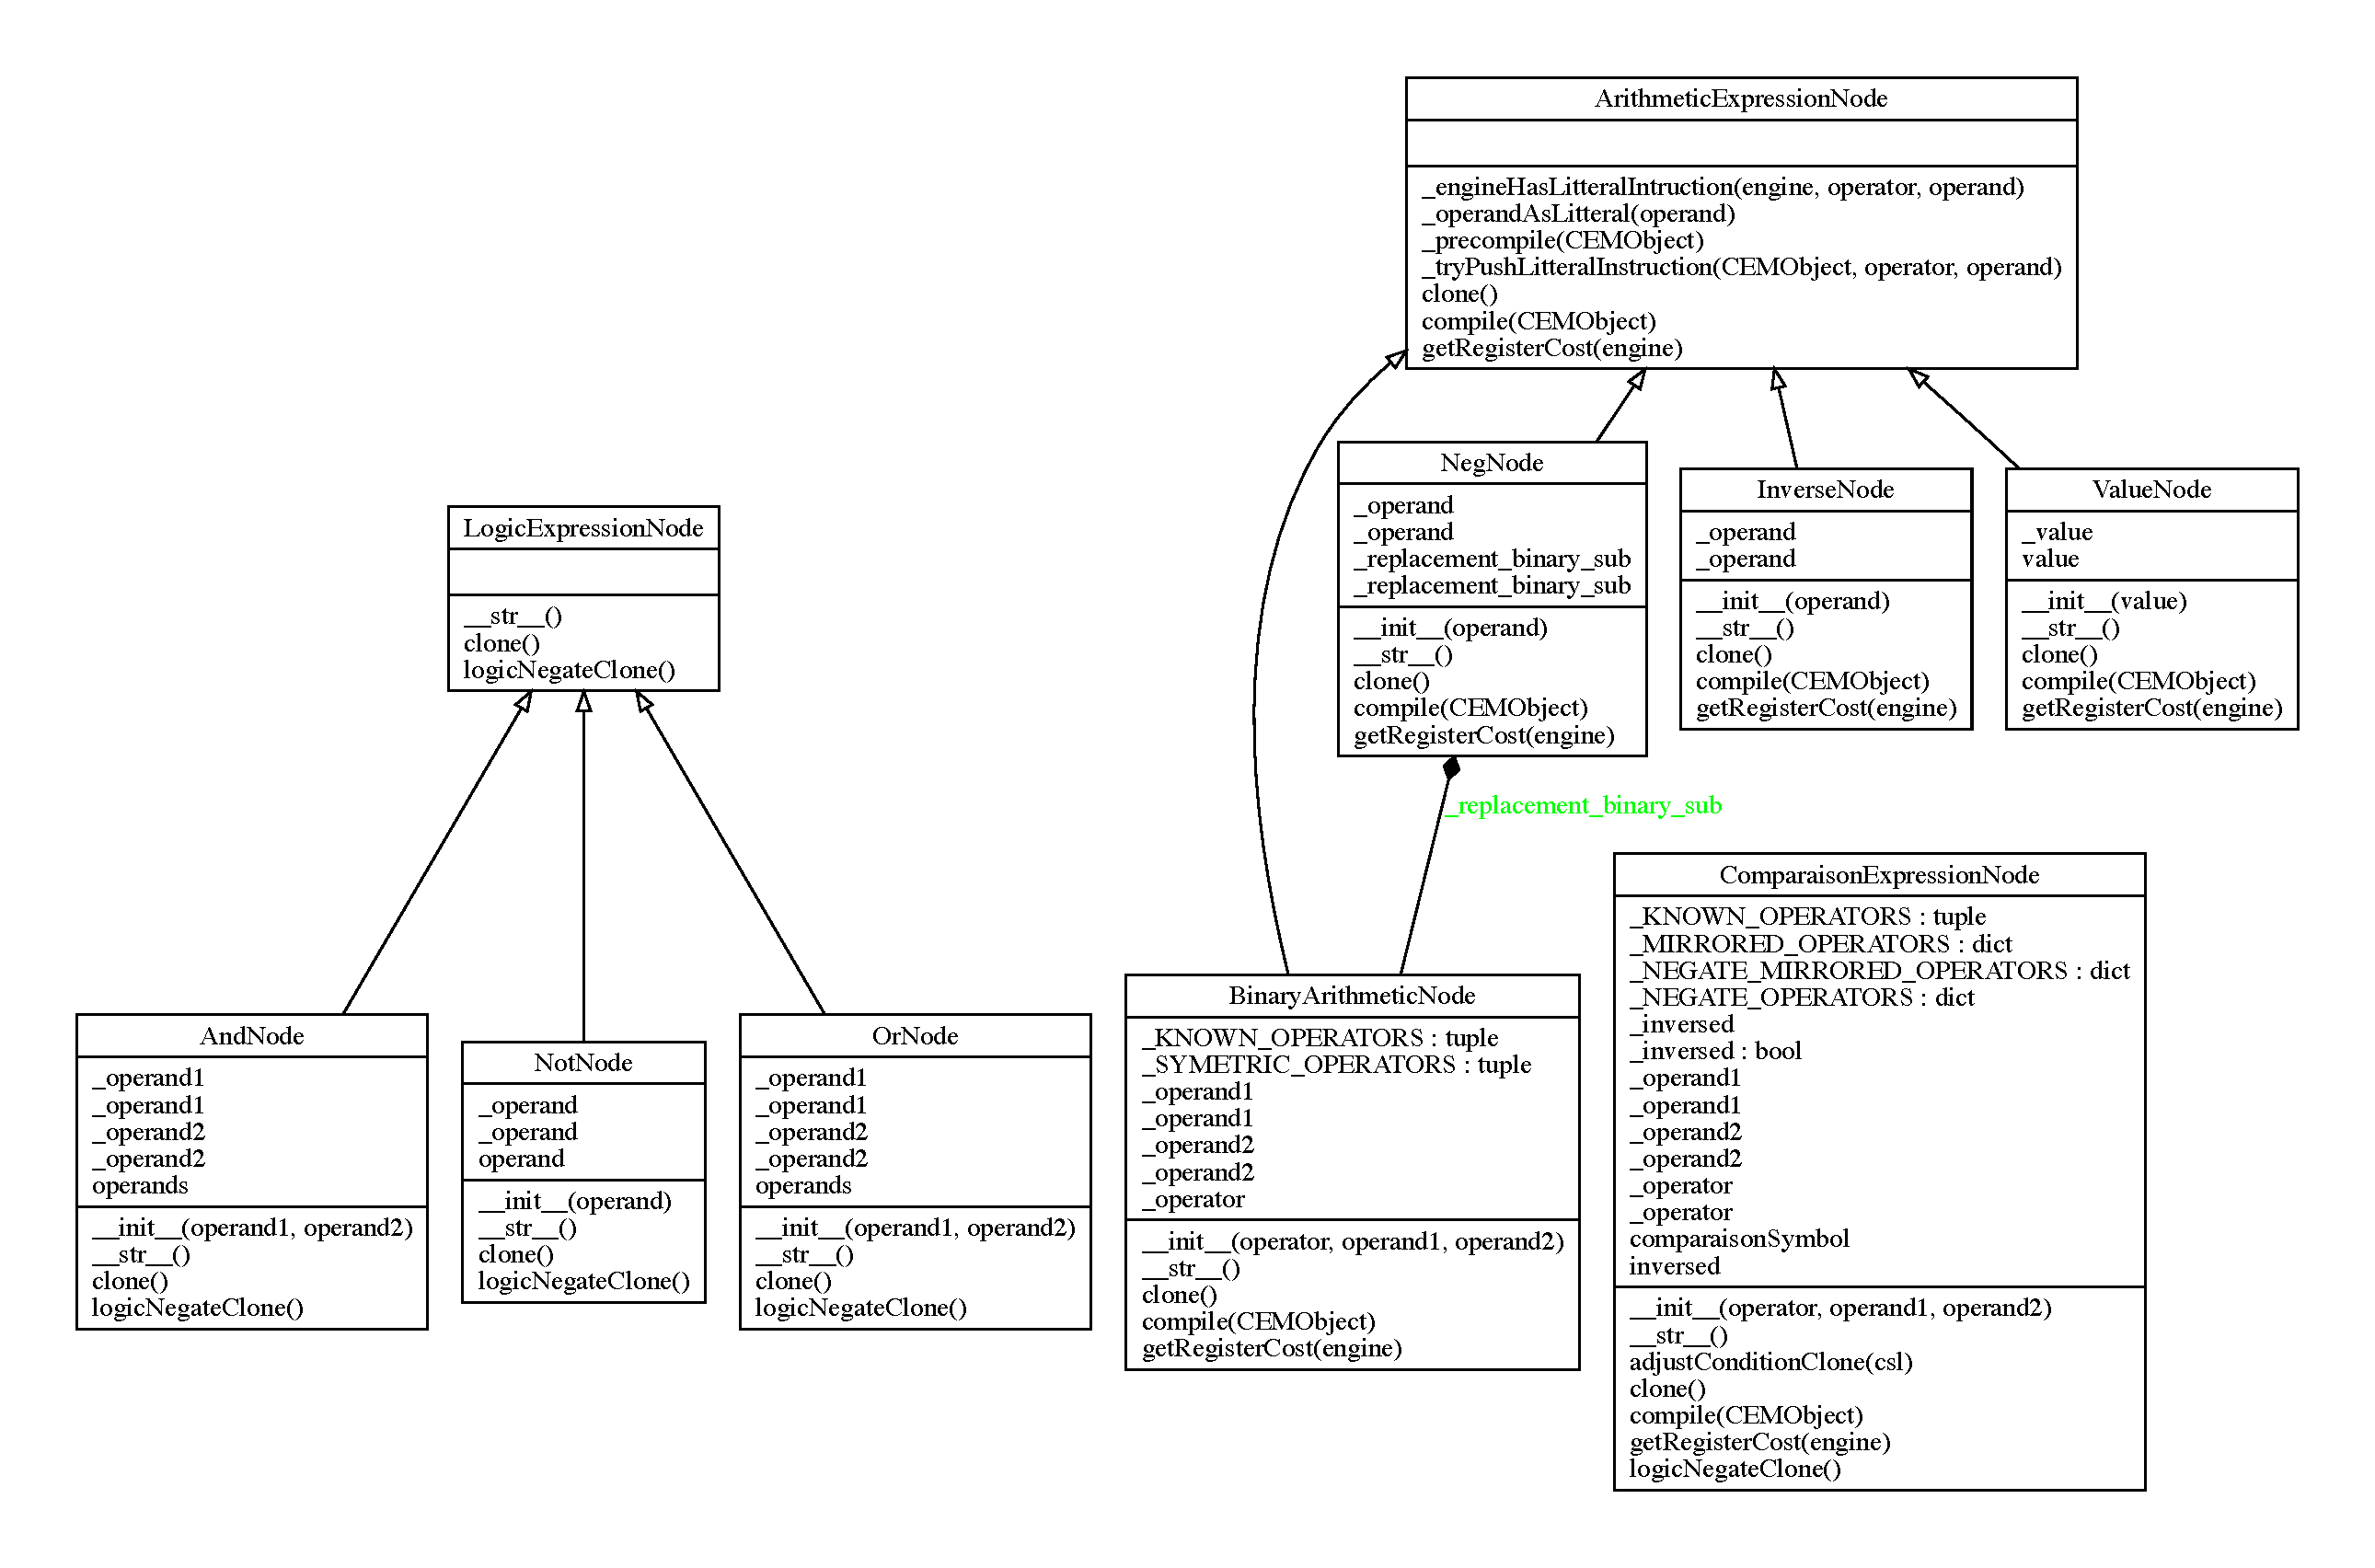
\includegraphics[width=\textwidth]{./Pictures/ExpressionNode.pdf}
	\caption{\label{fig:class_ExpressionNode}Diagramme de classes - ExpressionNode}
\end{figure}

Les expressions de type comparaisons (\pyinline{ComparisonExpressionNode}), expressions arithmétiques \pyinline{ArithmeticExpressionNode} ou les affectations (\pyinline{AffectationNode}) peuvent avoir pour attributs des instances de la classe \pyinline{ArithmeticExpressionNode}.


Une série de méthodes a été définie afin de pouvoir adapter l'expression de certaines conditions logiques aux propriétés du processeur (\ref{sec:processeur}). Par exemple, dans le cas où l'unité arithmétique et logique ne permet de tester que le caractère positif d'une valeur, une expression de type \pyinline{e1<e2} sera transformée en \pyinline{0 < e2-e1}. Les méthodes présentées renvoient une copie de l'expression initiale.

\begin{itemize}
	\item Négation logique d'une expression: \pyinline{logicNegateClone()}
	\item Adaptation des conditions: \pyinline{adjustConditionClone(csl)} avec \pyinline{csl} une liste de chaine de caractères correspondant aux symboles de comparaisons disponibles.

	\item \pyinline{negToSubClone()} transforme une expression de la forme \pyinline{-e} en \pyinline{0-e}.  
\end{itemize}
\begin{figure}[h!]
	\centering
	\begin{tikzpicture}
\begin{scope}
	\node[draw, minimum height=1.5em] (begin) at (0,0) {
		\texttt{\#4 > @x}
	};
	
	
	\node[right = 6cm of begin.east, draw, minimum height=1.5em] (end) {
		\texttt{@x < \#4}
	};
	
	\draw[->] (begin.east) -- (end) node[midway, above] {\pyinline{adjustConditionClone(['<', '=='])}};
\end{scope}

\begin{scope}[shift={(0,-1)}]
	\node[draw, minimum height=1.5em] (begin) at (0,0) {
		\texttt{\#8 >= @y}
	};
	
	
	\node[right = 6cm of begin.east, draw, minimum height=1.5em] (end) {
		\texttt{not (\#8 < @y)}
	};
	
	\draw[->] (begin.east) -- (end) node[midway, above] {\pyinline{adjustConditionClone(['<', '=='])}};
\end{scope}
	\end{tikzpicture}
	
	\caption{adjustConditionClone: exemples. Seuls les opérateurs \pyinline{<} et \pyinline{==} sont disponibles dans le modèle de processeur}
\end{figure}